
\documentclass[12pt]{article}

\usepackage{sbc-template}
\usepackage{graphicx,url}
\usepackage[utf8]{inputenc}
\usepackage[brazil]{babel}
\usepackage{listings}
\usepackage{xcolor}
\usepackage{float}
\usepackage{microtype}
\usepackage{amsmath}
\usepackage{multirow}

\sloppy

% Configuracao de estilo para listagens de codigo
\definecolor{codegreen}{rgb}{0,0.6,0}
\definecolor{codegray}{rgb}{0.5,0.5,0.5}
\definecolor{codepurple}{rgb}{0.58,0,0.82}
\definecolor{backcolour}{rgb}{0.97,0.97,0.97}

\lstdefinestyle{javastyle}{
  backgroundcolor=\color{backcolour},
  commentstyle=\color{codegreen}\itshape,
  keywordstyle=\color{blue}\bfseries,
  numberstyle=\tiny\color{codegray},
  stringstyle=\color{codepurple},
  basicstyle=\ttfamily\footnotesize,
  breakatwhitespace=false,
  breaklines=true,
  captionpos=b,
  keepspaces=true,
  numbers=left,
  numbersep=5pt,
  showspaces=false,
  showstringspaces=false,
  showtabs=false,
  tabsize=2,
  language=Java
}

\lstdefinestyle{sqlstyle}{
  backgroundcolor=\color{backcolour},
  commentstyle=\color{codegreen}\itshape,
  keywordstyle=\color{blue}\bfseries,
  numberstyle=\tiny\color{codegray},
  stringstyle=\color{codepurple},
  basicstyle=\ttfamily\footnotesize,
  breakatwhitespace=false,
  breaklines=true,
  captionpos=b,
  keepspaces=true,
  numbers=left,
  numbersep=5pt,
  showspaces=false,
  showstringspaces=false,
  showtabs=false,
  tabsize=2,
  language=SQL
}

\lstset{style=javastyle}

% -----------------------------------------------------------------------
\title{RootL: Um Motor de Change Data Capture Passivo Baseado em\\
  Arquitetura Hexagonal para Ambientes Governamentais Restritos}

\author{Leonardo de Oliveira Ramos\inst{1,2}}

\address{Instituto de Computação -- Universidade Federal de Mato Grosso (UFMT)\\
  Cuiabá -- MT -- Brasil
  \email{leonardo.ramos@sou.ufmt.br}
}

% -----------------------------------------------------------------------
\begin{document}

\maketitle

% -----------------------------------------------------------------------
\begin{abstract}
  Modern data architectures increasingly demand real-time integration
  pipelines from transactional databases into analytical platforms.
  However, in governmental environments, strict security policies prohibit
  the use of database triggers, the granting of broad administrative
  privileges, and the deployment of agents requiring direct write access
  to source databases. This paper presents \textbf{RootL CDC Publisher},
  a fully passive Change Data Capture (CDC) engine implemented in pure Java,
  designed to operate under such constraints. The proposed architecture
  adopts the Hexagonal (Ports \& Adapters) pattern to isolate the domain
  core from infrastructure concerns, enabling multi-database support
  (Oracle, PostgreSQL, MySQL) without modifying core processing logic.
  A SQL Abstract Syntax Tree (AST) parsing strategy based on JSqlParser
  is employed to reconstruct the complete row state (before/after) from
  Oracle LogMiner redo entries. Results demonstrate sub-second replication
  latency under normal conditions, with built-in resilience for log gap
  recovery and transactional consistency guaranteed by a commit-gated
  publication buffer.
\end{abstract}

\begin{resumo}
  Arquiteturas de dados modernas demandam pipelines de integração em tempo
  real a partir de bancos transacionais para plataformas analíticas. Em
  ambientes governamentais, políticas de segurança proíbem o uso de
  \textit{triggers}, a concessão de privilégios administrativos amplos e
  a implantação de agentes com acesso de escrita ao banco de origem. Este
  artigo apresenta o \textbf{RootL CDC Publisher}, um motor de Change Data
  Capture (CDC) 100\% passivo em Java puro, projetado para operar sob tais
  restrições. A arquitetura adota o padrão Hexagonal (\textit{Ports \&
  Adapters}) para isolar o núcleo de domínio, habilitando suporte multi-banco
  sem alterações na lógica central. Uma estratégia de \textit{parsing} de
  AST via JSqlParser reconstrói o estado completo da linha a partir dos
  registros de redo do Oracle LogMiner. Os resultados indicam latência
  sub-segundo, com mecanismos de resiliência para lacunas de log e
  consistência transacional garantida por buffer condicional ao
  \textit{commit}.
\end{resumo}


% -----------------------------------------------------------------------
\section{Introdução}
\label{sec:intro}

A crescente demanda por tomada de decisão orientada a dados em tempo real
impõe desafios significativos à integração entre sistemas transacionais
operacionais e plataformas analíticas, como Data Lakes e Data Warehouses.
A técnica de \textbf{Change Data Capture} (CDC) emerge como a abordagem
principal para capturar mutações em bancos de dados relacionais e propagá-las
de forma incremental e eficiente para sistemas \textit{downstream}
\cite{kleppmann:2017}.

Em ambientes corporativos convencionais, ferramentas consolidadas como
Oracle GoldenGate e Debezium oferecem soluções maduras para CDC. Contudo,
em \textbf{ambientes governamentais} com políticas de segurança rigorosas, tais como as vigentes em órgãos da administração pública brasileira,
a implantação dessas ferramentas enfrenta obstáculos que se mostraram, na
prática, intransponíveis. Equipes de governança de TI tipicamente proíbem:
(i) o uso de \textit{database triggers} para captura de eventos;
(ii) a concessão de privilégios amplos como \texttt{SELECT ANY TABLE};
(iii) a criação de \textit{replication slots} e o acesso ao catálogo
administrativo do banco de dados; e
(iv) qualquer instrução de escrita no banco de origem por parte da
ferramenta de integração.

Essas restrições inviabilizam tanto as soluções comerciais, cujo custo de
licenciamento é proibitivo para projetos de dados em fase de validação,
quanto as soluções \textit{open-source} mais disseminadas, que exigem
privilégios incompatíveis com os requisitos de governança vigentes.

Diante desse cenário, este trabalho apresenta o \textbf{RootL CDC Publisher},
um motor autônomo de CDC, 100\% passivo, desenvolvido em Java puro. O motor
conecta-se ao banco de dados e lê os logs transacionais nativos diretamente
em memória, sem executar nenhuma instrução de escrita, sem criar
\textit{triggers}, sem utilizar tabelas de controle e sem requerer DDLs
adicionais além da ativação pontual de \textit{supplemental logging} por
tabela monitorada. O sistema opera de forma transparente ao banco de origem.

A solução é estruturada sobre três pilares técnicos fundamentais:
(i) \textbf{Arquitetura Hexagonal} (\textit{Ports \& Adapters})
\cite{cockburn:2005}, que desacopla o núcleo de domínio dos adaptadores de
banco de dados e de publicação; (ii) \textbf{Parsing de AST do SQL de Redo}
via JSqlParser \cite{aho:2006}, para reconstrução do estado completo da
linha (\textit{before}/\textit{after}) em operações de UPDATE; e
(iii) \textbf{Buffer de Transação Condicional ao \textit{Commit}}, que
garante consistência transacional e impede que eventos de transações
revertidas contaminem o pipeline.

As principais contribuições deste trabalho são:
\begin{itemize}
  \item Proposição de uma arquitetura CDC passiva e multi-banco viável em
        ambientes de alta restrição de segurança;
  \item Mecanismo de reconstrução de \textit{Full State} via análise
        sintática (AST) do SQL de Redo do Oracle LogMiner;
  \item Estratégias de resiliência para falhas específicas do LogMiner
        (ORA-01289, ORA-01291) e para o \textit{Day 0 Problem};
  \item Modelo de configuração orientado a dados que elimina a necessidade
        de recompilação para adição de novas fontes de dados.
\end{itemize}

O restante deste artigo está organizado da seguinte forma: a
Seção~\ref{sec:related} discute os trabalhos relacionados; a
Seção~\ref{sec:arch} descreve a arquitetura hexagonal proposta; a
Seção~\ref{sec:challenges} detalha os desafios de implementação; a
Seção~\ref{sec:deployment} trata das considerações de implantação e
resiliência; a Seção~\ref{sec:eval} apresenta a avaliação experimental
de desempenho e latência; e a Seção~\ref{sec:conclusion} apresenta as
conclusões e trabalhos futuros.


% -----------------------------------------------------------------------
\section{Trabalhos Relacionados}
\label{sec:related}

A técnica de CDC é amplamente estudada e possui múltiplas abordagens de
implementação. \cite{kleppmann:2017} classifica os mecanismos de CDC em
três categorias: (i) baseados em \textit{triggers}; (ii) baseados em
consultas periódicas (\textit{timestamp-based polling}); e (iii) baseados
em logs transacionais (\textit{log-based CDC}). A abordagem baseada em
logs é considerada a mais eficiente e menos invasiva, por não introduzir
\textit{overhead} de escrita no banco de origem.

\subsection{Oracle GoldenGate}

O Oracle GoldenGate é a solução comercial de referência para captura e
replicação de dados em ambientes Oracle. Sua arquitetura opera no nível
do \textit{redo log} e suporta replicação heterogênea bidirecional com
latências mínimas. Contudo, a solução apresenta limitações críticas para
o contexto governamental: (i) seu custo de licenciamento por núcleo de
processador é elevado, tornando-o inviável para projetos de dados em
organizações públicas com orçamentos restritos; (ii) requer a instalação
de agentes proprietários (\textit{Extract} e \textit{Replicat}) no servidor
de banco de dados, o que viola políticas que proíbem softwares de terceiros
no ambiente de produção; e (iii) o modelo de licenciamento implica
dependência tecnológica de fornecedor único (\textit{vendor lock-in}).

\subsection{Debezium}

O Debezium \cite{debezium:2026} é a solução \textit{open-source} de CDC mais
amplamente adotada no ecossistema Apache Kafka. Para bancos Oracle, o Debezium
utiliza o LogMiner como mecanismo de extração, de forma análoga à abordagem
proposta neste trabalho. Entretanto, o conector Oracle do Debezium exige um
conjunto de permissões administrativas que inviabiliza sua adoção em ambientes
governamentais restritos: (i) \texttt{LOGMINING} combinado com
\texttt{SELECT ANY TABLE} para acessar os metadados do dicionário de dados;
(ii) acesso irrestrito às \textit{system views} do catálogo Oracle; e
(iii) em ambientes PostgreSQL, a criação de \textit{replication slots} de
decodificação lógica do WAL, considerados risco de segurança por equipes de
DBA em órgãos governamentais, pois retêm segmentos do WAL indefinidamente e
podem causar crescimento descontrolado de disco.

Além disso, o Debezium é implantado como conector do Kafka Connect, exigindo
toda a infraestrutura de \textit{workers} do Connect, o que aumenta a
complexidade operacional e o consumo de recursos em ambientes com restrições
de infraestrutura.

\subsection{Gap de Pesquisa e Posicionamento do RootL}

A Tabela~\ref{tab:comparison} sintetiza a comparação entre as abordagens
existentes e a solução proposta em relação aos critérios mais relevantes
para o contexto de ambientes governamentais restritos.

\begin{table}[H]
\centering
\caption{Comparação entre soluções de CDC para ambientes com restrições
  de segurança.}
\label{tab:comparison}
\begin{tabular}{|l|c|c|c|}
\hline
\textbf{Critério} & \textbf{GoldenGate} & \textbf{Debezium} & \textbf{RootL} \\
\hline
Custo & Licença comercial & Gratuito & Gratuito \\
\hline
Requer \texttt{SELECT ANY TABLE} & Não & Sim & Não \\
\hline
Requer \textit{replication slot} & Não & Sim (PG) & Não \\
\hline
Requer agente no servidor DB & Sim & Não & Não \\
\hline
Opera sem escrita no banco & Sim & Sim & Sim \\
\hline
Suporte multi-banco nativo & Sim & Sim & Sim \\
\hline
Configuração orientada a dados & Não & Parcial & Sim \\
\hline
Privilégio mínimo por tabela & Não & Não & Sim \\
\hline
\end{tabular}
\end{table}

O \textit{gap} central identificado é a ausência de uma solução
\textit{open-source} que combine: (i) leitura passiva via logs transacionais,
(ii) modelo de permissão estritamente granular por tabela, (iii) ausência
de qualquer instrução de escrita ou DDL global no banco de origem, e
(iv) arquitetura extensível sem recompilação. O RootL CDC Publisher é
proposto para preencher exatamente esse espaço.


% -----------------------------------------------------------------------
\section{Arquitetura Proposta}
\label{sec:arch}

\subsection{Visão Geral do Pipeline}

O sistema opera em um pipeline de duas fases sequenciais, conforme ilustrado
na Figura~\ref{fig:pipeline}.

\begin{figure}[H]
\centering
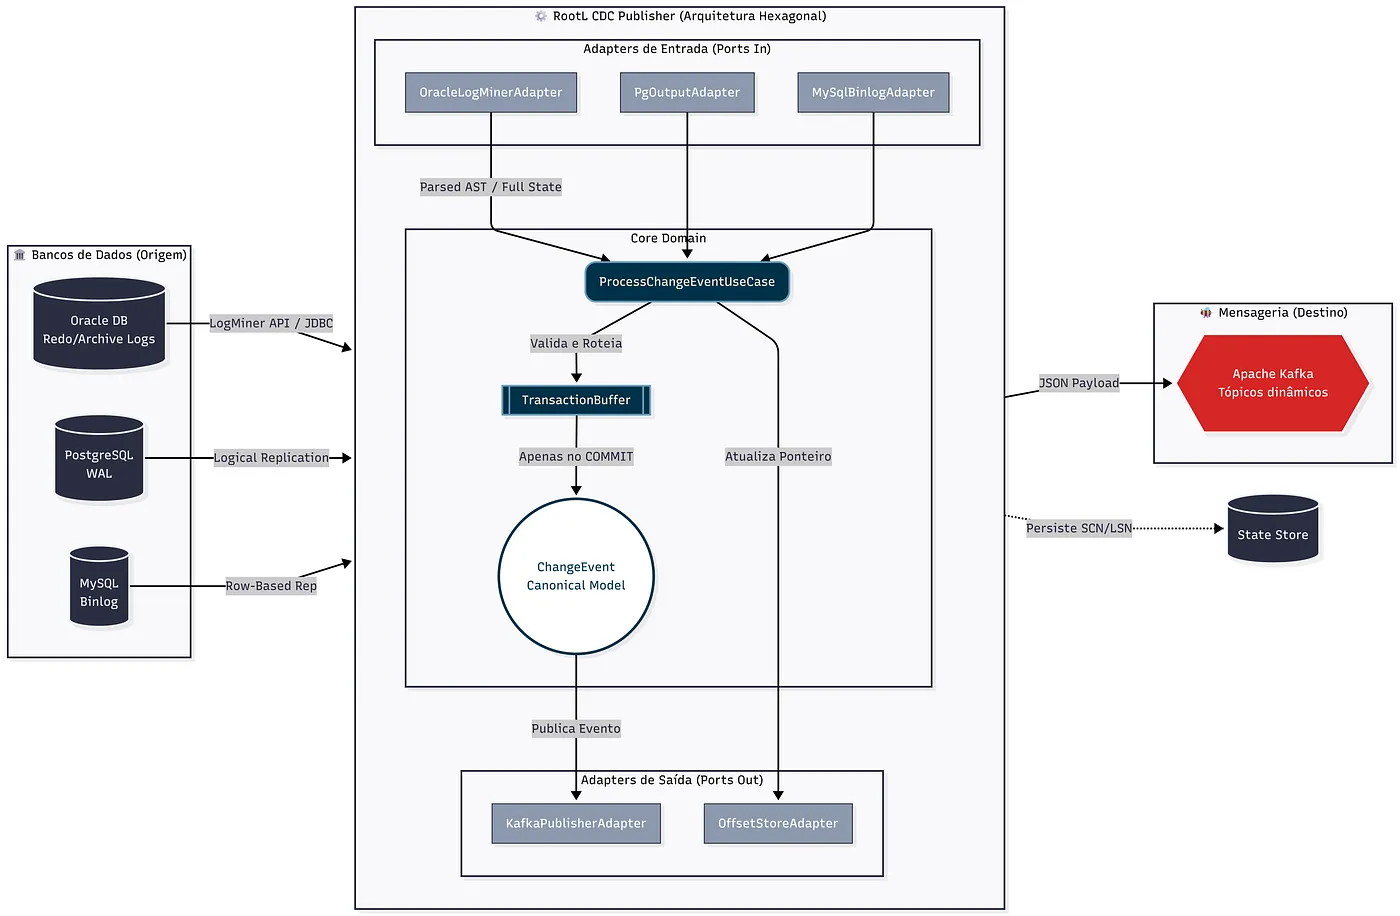
\includegraphics[width=0.95\textwidth]{figurasrootl/Fluxo-dos-dados (1).png}
\caption{Fluxo do pipeline de processamento do evento de mutação, da origem
  transacional ao tópico Apache Kafka.}
\label{fig:pipeline}
\end{figure}

A \textbf{Fase 1 - Extração Passiva} consiste na conexão ao banco de dados
e na leitura dos logs transacionais nativos sem a execução de qualquer
instrução de escrita. No Oracle, isso se materializa por meio da API do
LogMiner \cite{oracle:2023}, acessada via JDBC nativo, que permite varrer os
\textit{Redo Logs} e \textit{Archive Logs} e obter as instruções SQL de redo
correspondentes a cada evento DML (\texttt{INSERT}, \texttt{UPDATE},
\texttt{DELETE}).

A \textbf{Fase 2 - Normalização e Publicação} traduz cada mutação capturada
para um modelo canônico (\texttt{ChangeEvent}) e o publica como documento
JSON no Apache Kafka \cite{kleppmann:2017}, com roteamento dinâmico de
tópicos baseado no identificador do conector, no esquema e na tabela de
origem (e.g., \texttt{cdc.oracle-rh.RH.FUNCIONARIOS}).

\subsection{A Arquitetura Hexagonal como Princípio Fundamental}
\label{subsec:hex}

A decisão arquitetural central do RootL CDC Publisher é a adoção do padrão
\textbf{Arquitetura Hexagonal} (\textit{Ports \& Adapters})
\cite{cockburn:2005}. Concebido por Alistair Cockburn, esse padrão preconiza
a separação estrita entre o núcleo de domínio da aplicação e os mecanismos
de entrada e saída (I/O), de modo que o domínio expresse apenas \textit{o que}
o sistema deve fazer, delegando o \textit{como} para adaptadores
intercambiáveis.

No contexto do RootL, essa escolha é estratégica por três razões:
(i) o motor precisa suportar múltiplos bancos de dados (Oracle, PostgreSQL,
MySQL) e múltiplos destinos de publicação (Kafka hoje, possivelmente Apache
Pulsar ou RabbitMQ no futuro); (ii) a adição de um novo banco não deve
exigir alterações na lógica de processamento central; e (iii) o núcleo de
domínio deve ser testável de forma isolada, sem dependência de qualquer banco
ou \textit{broker} de mensagens.

\subsubsection{O Modelo Canônico: \texttt{ChangeEvent}}

No coração do sistema, o \texttt{ChangeEvent} é o modelo para o qual todas
as fontes devem convergir. Independentemente de o evento ter originado de
um \textit{Redo Log} Oracle, de um WAL PostgreSQL ou de um Binlog MySQL,
o formato de saída é sempre o mesmo. A Listagem~\ref{lst:changeevent}
apresenta a definição do \textit{record} imutável em Java.

\begin{lstlisting}[style=javastyle,
  caption={Modelo canônico \texttt{ChangeEvent} e tipos auxiliares.},
  label={lst:changeevent}]
public record ChangeEvent(
    UUID eventId,
    OperationType operation,
    Instant timestamp,
    SourceMetadata source,
    Map<String, Object> before,
    Map<String, Object> after) {

  public ChangeEvent {
    if (eventId == null)
      throw new IllegalArgumentException("eventId nao pode ser nulo");
    if (operation == null)
      throw new IllegalArgumentException("operation nao pode ser nula");
    if (source == null)
      throw new IllegalArgumentException("source nao pode ser nulo");
  }
}

public enum OperationType {
  INSERT, UPDATE, DELETE, BEGIN, COMMIT, READ
}

public record SourceMetadata(
    String connectorName,   String connectorType,
    String database,        String schema,
    String table,           String transactionId,
    Map<String, String> offsetCoordinates) {}
\end{lstlisting}

Cada \texttt{ChangeEvent} carrega: (i) um \texttt{eventId} UUID v4 para
rastreabilidade e deduplicação \textit{downstream}; (ii) a
\texttt{operation}, que representa o ciclo transacional completo
(\texttt{BEGIN}, \texttt{INSERT/UPDATE/DELETE}, \texttt{COMMIT}), sendo
\texttt{BEGIN} e \texttt{COMMIT} fundamentais para o funcionamento do
\texttt{TransactionBuffer}; (iii) os metadados de rastreio em
\texttt{SourceMetadata}, incluindo as coordenadas de \textit{offset}
(SCN para Oracle, LSN para PostgreSQL, posição de Binlog para MySQL); e
(iv) os mapas \texttt{before} e \texttt{after}, que representam a fotografia
completa da linha antes e após a mutação.

\subsubsection{Os \textit{Ports}: Contratos de Infraestrutura}

A interface \texttt{ChangeLogConnector} define o contrato que todo adaptador
de banco de dados deve implementar, conforme a Listagem~\ref{lst:port}.

\begin{lstlisting}[style=javastyle,
  caption={Interface \texttt{ChangeLogConnector}, \textit{port} de entrada.},
  label={lst:port}]
public interface ChangeLogConnector {
  void initialize(String connectorId, Properties config,
      ProcessChangeEventUseCase useCase,
      OffsetStorePort offsetStore,
      MeterRegistry meterRegistry);
  void start();
  void stop();
  String getType();
}
\end{lstlisting}

Do lado de saída (\textit{driven ports}), dois contratos governam
respectivamente a publicação de eventos e o armazenamento de estado de
\textit{offset}:

\begin{lstlisting}[style=javastyle,
  caption={\textit{Ports} de saída: publicação de eventos e armazenamento de \textit{offset}.},
  label={lst:outports}]
public interface EventPublisherPort {
  void publish(ChangeEvent event);
  void close();
}

public interface OffsetStorePort {
  void save(String connectorId, String lsn);
  Optional<String> load(String connectorId);
}
\end{lstlisting}

Essa separação garante que o caso de uso central
(\texttt{ProcessChangeEventUseCase}) jamais conhece a tecnologia por trás
da publicação ou do armazenamento de estado. Ele opera exclusivamente sobre
os contratos. A consequência direta é que, quando suporte a MySQL e
PostgreSQL foi adicionado ao motor, nenhuma linha do
\texttt{ProcessChangeEventUseCase} foi modificada. Foram criados novos
adaptadores implementando \texttt{ChangeLogConnector}, e o motor passou a
suportar as novas fontes de dados automaticamente, sem recompilação do
núcleo.

\subsubsection{Orquestração por Dados: Conectores como Configuração JSON}

A instanciação dos adaptadores é governada por arquivos JSON na pasta
\texttt{/connectors}. A aplicação varre o diretório no \textit{startup},
instancia os adaptadores via reflexão e os registra no \texttt{CdcEngine}.
Adicionar um novo banco de dados é, portanto, uma operação de configuração,
não de engenharia: o DBA provisiona as permissões, a equipe de DevOps cria
o arquivo JSON, e o contêiner sobe consumindo o novo fluxo sem necessidade
de recompilação.

\subsection{O \texttt{TransactionBuffer}: Garantia de Consistência Transacional}

Uma decisão de projeto considerada crítica para a integridade dos dados é o
\texttt{TransactionBuffer}: eventos de mutação não são publicados
imediatamente no Kafka. Eles são retidos em um buffer em memória
(\texttt{ConcurrentHashMap}) agrupados por \texttt{transactionId}, e somente
liberados quando o sinal de \texttt{COMMIT} é recebido.

A motivação é clara: o LogMiner (e o WAL do PostgreSQL) transmitem eventos DML
\textit{antes} da confirmação da transação. Se um usuário executa um
\texttt{INSERT} seguido de \texttt{ROLLBACK}, esse \texttt{INSERT} já foi
transmitido pelo log. Sem o buffer, o dado fantasma alcançaria o Kafka e
eventualmente o Data Lake. Com o \texttt{TransactionBuffer}, \textit{rollbacks}
são descartados de forma determinística. A Listagem~\ref{lst:txbuffer}
apresenta a implementação central.

\begin{lstlisting}[style=javastyle,
  caption={Implementação do \texttt{TransactionBuffer} com limite de eventos por transação.},
  label={lst:txbuffer}]
public class TransactionBuffer {
  private static final int MAX_EVENTS_PER_TX = 10_000;
  private final Map<String, List<ChangeEvent>> buffer =
      new ConcurrentHashMap<>();

  public void addEvent(String transactionId, ChangeEvent event) {
    buffer.compute(transactionId, (txId, events) -> {
      if (events == null) events = new ArrayList<>();
      if (events.size() < MAX_EVENTS_PER_TX) events.add(event);
      return events;
    });
  }

  public List<ChangeEvent> commit(String transactionId) {
    List<ChangeEvent> events = buffer.remove(transactionId);
    return events != null ? events : List.of();
  }

  public void rollback(String transactionId) {
    buffer.remove(transactionId);
  }
}
\end{lstlisting}

O limite \texttt{MAX\_EVENTS\_PER\_TX} (10.000 eventos) protege o motor
contra transações de larga escala (\textit{bulk loads}) que poderiam causar
pressão de memória. A regra de publicação é inequívoca: \textit{somente
publica no Kafka o que sobrevive ao COMMIT}.

\subsection{O \texttt{CdcEngine}: Orquestração do Ciclo de Vida}

O \texttt{CdcEngine} é o orquestrador central do motor. Ele gerencia o
ciclo de vida dos conectores, executando cada um em sua própria
\textit{thread} isolada por meio de um \texttt{CachedThreadPool}. Em caso
de falha de um conector (e.g., banco Oracle indisponível), os demais
continuam operando normalmente. O \textit{shutdown} é gerenciado com janela
de 30 segundos para finalização segura das transações em andamento, após
o qual um encerramento forçado é executado para garantir que o processo
seja terminado de forma limpa.


% -----------------------------------------------------------------------
\section{Desafios de Implementação}
\label{sec:challenges}

\subsection{Navegação Multitenant e o Princípio do Privilégio Mínimo}

Na arquitetura Multitenant do Oracle 12c+, os \textit{Redo Logs} são físicos
e residem no Container Database (CDB), enquanto os dados de negócio habitam
os Pluggable Databases (PDBs) \cite{oracle:2023}. Para ler mutações de um
PDB específico, é necessário operar no nível do CDB, o que, superficialmente,
parece exigir privilégios administrativos amplos.

A solução adotada é a criação de um \textit{Common User} (\texttt{C\#\#CDC\_USER})
com permissões estritamente granulares, conforme a Listagem~\ref{lst:grants}.
A separação de responsabilidades é central: as permissões no CDB são de
\textit{infraestrutura} (acesso aos logs físicos), enquanto as permissões
no PDB são de \textit{dados} e restritas às tabelas-alvo individualmente.
O \texttt{SELECT ANY TABLE}, o principal ponto de controvérsia em
auditorias de segurança, é completamente eliminado.

\begin{lstlisting}[style=sqlstyle,
  caption={Concessão de privilégios mínimos para o usuário CDC no Oracle Multitenant.},
  label={lst:grants}]
-- Ativacao do supplemental logging por tabela (nao global)
ALTER TABLE RH.FUNCIONARIOS ADD SUPPLEMENTAL LOG DATA (ALL) COLUMNS;

-- Permissoes de infraestrutura no CDB (nao de dados)
GRANT CREATE SESSION, ALTER SESSION, SET CONTAINER
  TO C##CDC_USER CONTAINER=ALL;
GRANT LOGMINING TO C##CDC_USER CONTAINER=ALL;
GRANT SELECT ANY TRANSACTION TO C##CDC_USER CONTAINER=ALL;
GRANT EXECUTE ON SYS.DBMS_LOGMNR TO C##CDC_USER CONTAINER=ALL;
GRANT SELECT ON SYS.V_$LOGMNR_CONTENTS TO C##CDC_USER CONTAINER=ALL;
GRANT SELECT ON SYS.V_$LOG, SYS.V_$LOGFILE TO C##CDC_USER CONTAINER=ALL;
GRANT SELECT ON SYS.V_$ARCHIVED_LOG TO C##CDC_USER CONTAINER=ALL;

-- Permissao de dados apenas nas tabelas-alvo no PDB especifico
ALTER SESSION SET CONTAINER = ORCHET1;
GRANT SELECT ON RH.FUNCIONARIOS TO C##CDC_USER;
GRANT SELECT ON RH.CONTRATOS TO C##CDC_USER;
\end{lstlisting}

A sessão JDBC é fixada no \texttt{CDB\$ROOT} para acessar os logs físicos
globais. A consulta ao \texttt{V\$LOGMNR\_CONTENTS} aplica filtro pela
coluna \texttt{SRC\_CON\_NAME}, garantindo que o usuário CDC visualize
exclusivamente os dados do PDB autorizado, nunca os de outros
\textit{containers} na mesma instância CDB. Esse mecanismo é ilustrado
na Figura~\ref{fig:jdbc}.

\begin{figure}[H]
\centering
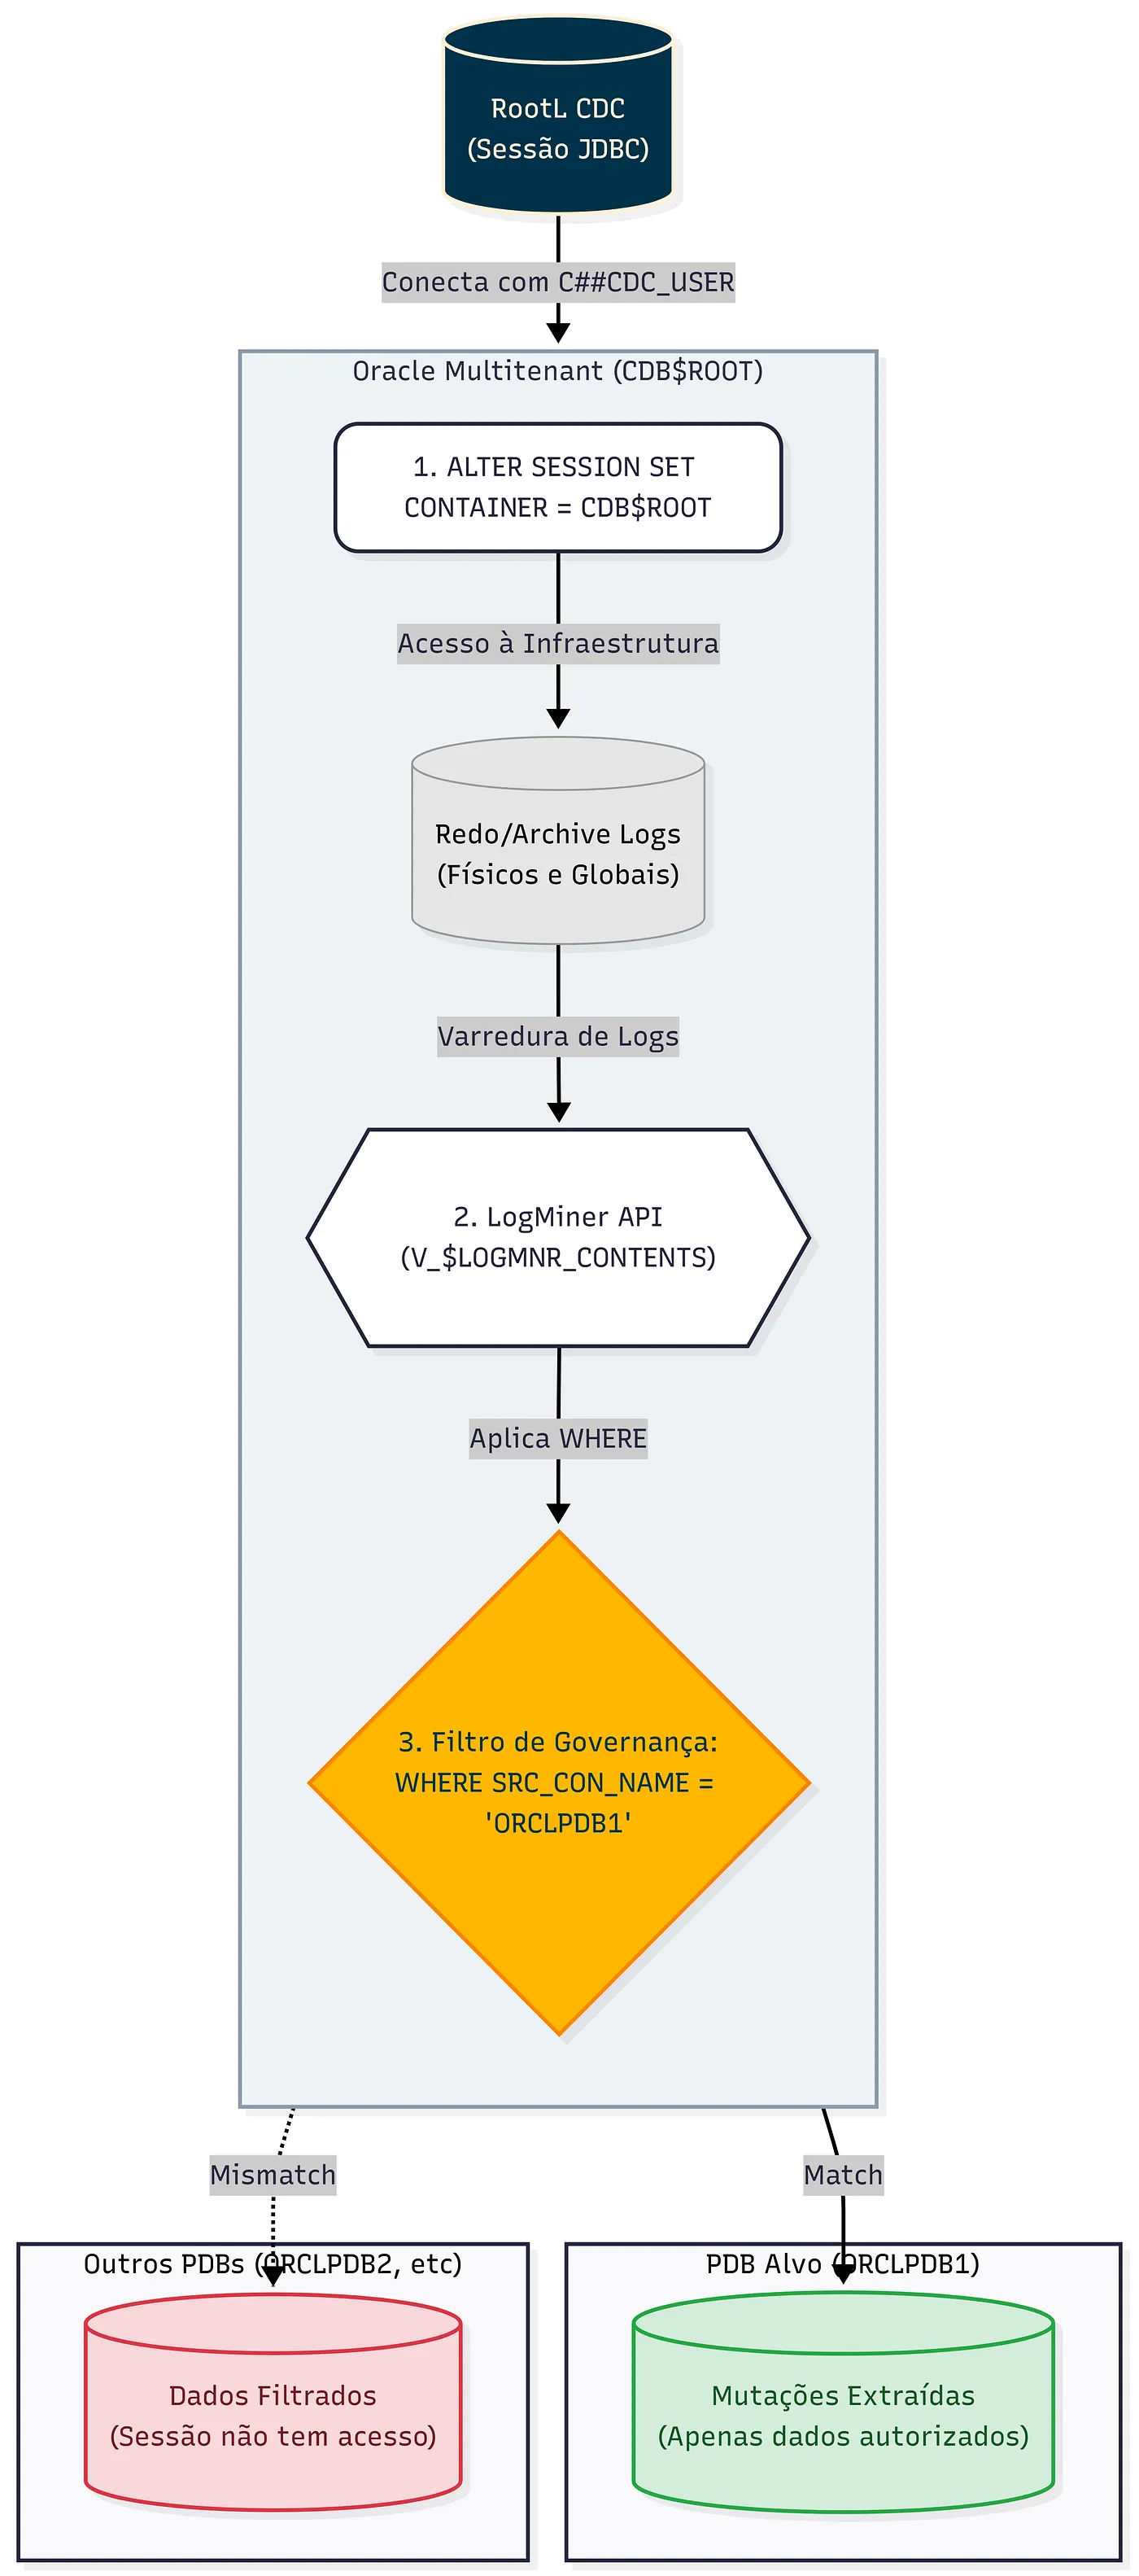
\includegraphics[width=0.60\textwidth]{figurasrootl/Fluxo-de-gestao-jdbc (1).png}
\caption{Fluxo de gestão da sessão JDBC no ambiente Oracle Multitenant:
  a sessão é fixada no CDB para leitura dos logs físicos, mas a consulta
  ao \texttt{V\$LOGMNR\_CONTENTS} filtra dados pelo PDB de origem via
  \texttt{SRC\_CON\_NAME}.}
\label{fig:jdbc}
\end{figure}

\subsection{O Problema do Estado Completo (\textit{Full State}) e o JSqlParser}
\label{subsec:fullstate}

Um dos desafios mais sutis e tecnicamente ricos do motor reside na
reconstrução do estado completo da linha em operações de UPDATE. O Oracle,
por razões de eficiência de I/O, não registra o registro inteiro no Redo Log
em mutações de UPDATE, registra apenas o \textit{delta}, ou seja,
as colunas modificadas. O SQL de Redo resultante tem o seguinte formato:

\begin{lstlisting}[style=sqlstyle,
  caption={SQL de Redo gerado pelo Oracle LogMiner para uma operação de UPDATE.},
  label={lst:redosql}]
UPDATE "RH"."FUNCIONARIOS"
SET "CARGO" = 'Analista'
WHERE "ID" = '158'
  AND "NOME" = 'Leonardo Ramos'
  AND "CARGO" = 'Estagiario'
  AND "DEPARTAMENTO" = 'Inteligencia';
\end{lstlisting}

Observa-se que a cláusula \texttt{SET} contém apenas o campo alterado, enquanto
a cláusula \texttt{WHERE} contém \textit{todas} as colunas da linha, esse
é o \textit{Before Image} garantido pelo Supplemental Logging
\cite{oracle:2023}. Para que o pipeline \textit{downstream} possa consumir
um evento de CDC semanticamente completo, são necessários dois objetos
distintos: o \texttt{before} (estado pré-mutação completo) e o \texttt{after}
(estado pós-mutação completo).

\subsubsection{Parsing de AST e o Padrão \textit{Visitor}}

A solução aplica os princípios da teoria de compiladores \cite{aho:2006}
para analisar o SQL de Redo como uma Árvore Sintática Abstrata (AST).
O JSqlParser decompõe a instrução SQL em uma hierarquia de nós tipados
(\texttt{Update}, \texttt{AndExpression}, \texttt{EqualsTo},
\texttt{IsNullExpression}, \texttt{ExpressionList}, entre outros), sobre
a qual um algoritmo recursivo baseado no padrão \textit{Visitor} navega
para extrair os dados de interesse.

O padrão \textit{Visitor} é especialmente adequado para esse problema porque
permite desacoplar o algoritmo de extração da estrutura da árvore: cada tipo
de nó da AST é processado por uma função específica, sem necessidade de
modificar as classes do parser. O \textit{Visitor} percorre a árvore binária
de expressões, terminando a recursão nas folhas (\texttt{EqualsTo} e
\texttt{IsNullExpression}), onde os pares coluna/valor são extraídos
\cite{aho:2006}. A Listagem~\ref{lst:visitor} apresenta o método recursivo
central.

\begin{lstlisting}[style=javastyle,
  caption={Extração recursiva do \textit{Before Image} via padrão \textit{Visitor} sobre a AST.},
  label={lst:visitor}]
private static void extractColumnsFromWhereClause(
    Expression expr, Map<String, Object> beforeMap) {

  if (expr instanceof AndExpression and) {
    // Recursao: desce nos dois ramos da arvore binaria
    extractColumnsFromWhereClause(and.getLeftExpression(), beforeMap);
    extractColumnsFromWhereClause(and.getRightExpression(), beforeMap);

  } else if (expr instanceof EqualsTo equals) {
    // Folha: extrai o par coluna=valor
    String colName = equals.getLeftExpression()
        .toString().replace("\"", "").toUpperCase();
    String colValue = equals.getRightExpression()
        .toString().replaceAll("^'|'$", "");
    beforeMap.put(colName,
        "NULL".equalsIgnoreCase(colValue) ? null : colValue);

  } else if (expr instanceof IsNullExpression isNull) {
    // Caso especial: colunas NULL nao geram EqualsTo na AST
    String colName = isNull.getLeftExpression()
        .toString().replace("\"", "").toUpperCase();
    beforeMap.put(colName, null);
  }
}
\end{lstlisting}

O algoritmo completo de reconstrução de \textit{Full State} opera em três
etapas sequenciais: (i) \textbf{Parse} do SQL de Redo via
\texttt{CCJSqlParserUtil.parse()}, obtendo a AST da instrução
\texttt{Update}; (ii) \textbf{Extração do \textit{Before}}: navegação
recursiva pela cláusula \texttt{WHERE} da AST, construindo o mapa
\texttt{before} com o estado pré-mutação completo; e
(iii) \textbf{Construção do \textit{After}}: clonagem integral de
\texttt{before} para \texttt{after}, seguida de sobrescrita apenas das
colunas presentes na cláusula \texttt{SET}.

O resultado é um payload JSON de \textit{Full State} que permite ao
consumidor \textit{downstream} identificar com precisão exatamente quais
colunas foram alteradas. \textbf{Pré-requisito crítico}: essa estratégia
é dependente da ativação do \textit{Supplemental Logging} nas tabelas-alvo
(\texttt{ALL COLUMNS}). Sem essa configuração, o Oracle omite a cláusula
\texttt{WHERE} detalhada do SQL de Redo, registrando apenas a \texttt{ROWID},
tornando o \textit{Before Image} irrecuperável. A ativação deve ser feita
por tabela individualmente, não globalmente, para evitar
\textit{overhead} desnecessário de I/O em esquemas com grande número de
tabelas.

\subsection{Deduplicação por \textit{Fingerprinting}}
\label{subsec:dedup}

O LogMiner apresenta um comportamento inerente que pode causar reprocessamento
de eventos: ao consultar com \texttt{SCN >= ?}, o motor pode retornar eventos
já processados no ciclo anterior, pois o SCN marca o \textit{commit} de uma
transação inteira, não de um registro individual. Para neutralizar esse
comportamento, é mantido um cache de \textit{fingerprints} que combina quatro
dimensões do evento: a operação, a tabela, o \texttt{ROWID} e o SQL de Redo
completo. O cache é purgado quando o SCN avança, garantindo que a memória
não cresça indefinidamente. Esse mecanismo garante idempotência no
processamento sem a necessidade de consultar sistemas externos para verificar
duplicatas.


% -----------------------------------------------------------------------
\section{Considerações de Implantação e Resiliência}
\label{sec:deployment}

\subsection{Tratamento de Erros Específicos do LogMiner}

O Oracle LogMiner, embora poderoso, expõe um conjunto de comportamentos de
erro que devem ser tratados explicitamente por um motor de CDC de nível
enterprise \cite{oracle:2023}. Dois erros são particularmente críticos:

\subsubsection{ORA-01289: Log File Already Added}

Em ambientes com espelhamento de disco (ASM ou sistemas de arquivos com
múltiplos membros por grupo de log), o mesmo arquivo de log pode aparecer
mais de uma vez nas \textit{views} de catálogo. Tentativas de adicionar
um arquivo já registrado na sessão do LogMiner resultam no erro
\texttt{ORA-01289}. A solução adotada é a captura da exceção com tratamento
silencioso (\textit{graceful ignore}), mantendo a \textit{flag}
\texttt{logFilesAdded = true}. Essa abordagem é operacionalmente segura,
pois o arquivo já foi registrado e a sessão continua válida.

\subsubsection{ORA-01291: Missing Log File}

Este erro é consideravelmente mais grave. Ele ocorre quando o RMAN executa
um expurgo agressivo de Archive Logs e remove um arquivo que o motor ainda
precisaria para ler a partir do SCN salvo no \textit{offset store}. A
estratégia de autocorreção implementada: (i) detecta o erro; (ii) consulta
o SCN mais recente disponível no servidor via \texttt{V\$LOG}; (iii) avança
o ponteiro de \textit{offset} para esse novo SCN; (iv) limpa o cache de
\textit{fingerprints}; e (v) retoma a mineração. A lacuna temporal é
registrada em métricas Prometheus para análise posterior. O sistema não
entra em estado de falha nem exige intervenção manual.

\subsubsection{\textit{Gap Detection} Proativo}

Além do tratamento reativo, o motor implementa uma verificação proativa de
lacunas de SCN a cada ciclo de mineração, consultando o
\texttt{MIN(FIRST\_CHANGE\#)} dos Archive Logs disponíveis. Caso o SCN
atual do \textit{offset} seja anterior ao log mais antigo disponível, o
motor emite um alerta de severidade crítica, avança o ponteiro
automaticamente e retoma a operação. Esse comportamento diferencia um
protótipo de um motor enterprise: \textit{o sistema detecta o buraco,
adapta-se e continua operando}.

\subsection{O \textit{Day 0 Problem}: Consistência do Snapshot Inicial}

Todo motor de CDC enfrenta um problema fundamental na data de implantação:
o streaming de logs captura apenas mutações \textit{futuras}. Os dados
preexistentes no banco são invisíveis ao motor. A solução é o
\textbf{Snapshot Inicial}, uma carga integral dos registros existentes antes
do início do streaming \cite{kleppmann:2017}.

O desafio é garantir consistência de ponto no tempo: se durante a leitura
do snapshot um registro for modificado, esse registro deve aparecer no
snapshot \textit{ou} no stream, nunca nos dois (duplicata) nem em nenhum
(perda). A estratégia varia por banco de dados:

\begin{itemize}
  \item \textbf{PostgreSQL}: utiliza \texttt{TRANSACTION\_REPEATABLE\_READ}
        com \texttt{setReadOnly(true)}, que congela a visão dos dados sem
        aplicar locks de escrita. O LSN atual é capturado via
        \texttt{pg\_current\_wal\_lsn()} e salvo como \textit{offset} base.
        Quando o snapshot é concluído, o streaming inicia exatamente a partir
        desse LSN, garantindo costura perfeita sem sobreposição.
  \item \textbf{Oracle}: utiliza \textit{Flashback Query}
        (\texttt{AS OF SCN}) na camada \textit{downstream}, consultando as
        tabelas em um SCN congelado. O motor de streaming, quando não encontra
        \textit{offset} salvo, obtém o \texttt{FIRST\_CHANGE\#} do Redo Log
        ativo e o usa como SCN de partida.
  \item \textbf{MySQL}: aplica \texttt{FLUSH TABLES WITH READ LOCK}, captura
        a posição do Binlog via \texttt{SHOW MASTER STATUS}, inicia a transação
        com \texttt{START TRANSACTION WITH CONSISTENT SNAPSHOT} e libera o
        lock imediatamente. A janela de lock é reduzida à ordem de
        milissegundos.
\end{itemize}

A metáfora é precisa: o snapshot é a \textbf{fotografia} e o stream é o
\textbf{vídeo}. A fotografia é tirada no exato frame onde o vídeo começa.

\subsection{Observabilidade: Métricas de Produção}

O RootL CDC Publisher expõe métricas nativas via Micrometer no
\textit{endpoint} \texttt{/actuator/prometheus}, prontas para coleta pelo
Prometheus e visualização no Grafana. A Figura~\ref{fig:metrics} apresenta
as principais métricas monitoradas.

\begin{figure}[H]
\centering
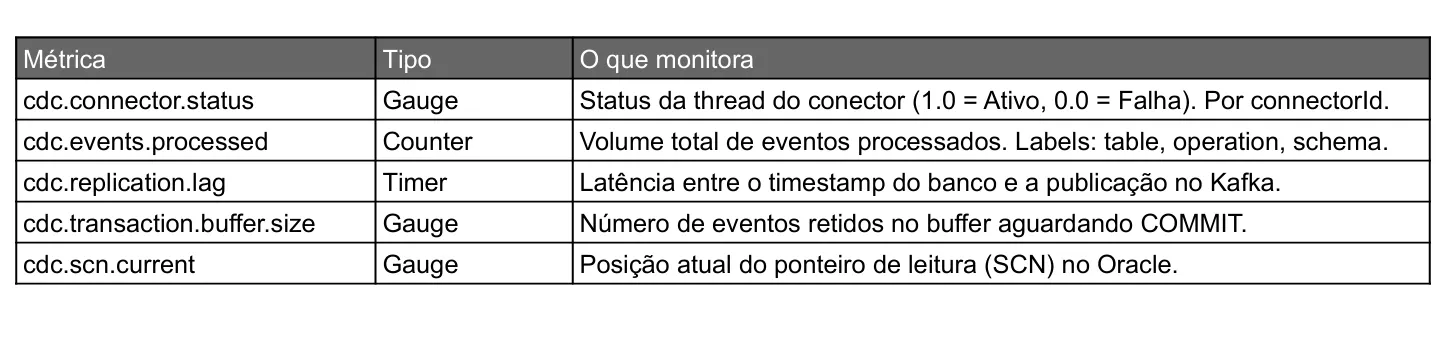
\includegraphics[width=0.82\textwidth]{figurasrootl/principais-metricas.png}
\caption{Principais métricas expostas pelo RootL CDC Publisher via
  Micrometer/Prometheus, incluindo a latência de replicação
  (\texttt{cdc.replication.lag}).}
\label{fig:metrics}
\end{figure}

A métrica \texttt{cdc.replication.lag} é particularmente relevante: ela
mede o delta entre o \texttt{TIMESTAMP} do SQL de Redo e o momento em que
o evento entra no buffer de publicação. Em condições operacionais normais,
esse valor se mantém consistentemente abaixo de 1 segundo, satisfazendo o
requisito de integração em sub-segundo estabelecido como meta do sistema.

\subsection{Suporte Multi-Banco: Um Motor, Três Ecossistemas}

A Arquitetura Hexagonal habilita o RootL a suportar três ecossistemas de
banco de dados simultaneamente, cada um com sua mecânica nativa de captura
de logs. Cada adaptador executa em sua própria \textit{thread} isolada,
gerenciada pelo \texttt{CdcEngine} com um \texttt{CachedThreadPool}.
A Tabela~\ref{tab:adapters} sumariza as estratégias por banco de dados.

\begin{table}[H]
\centering
\caption{Estratégias de captura de log por adaptador de banco de dados.}
\label{tab:adapters}
\begin{tabular}{|l|l|l|l|}
\hline
\textbf{Banco} & \textbf{Mecanismo} & \textbf{Offset} & \textbf{Adaptador} \\
\hline
Oracle & LogMiner (\textit{Redo Log}) & SCN & \texttt{OracleLogMinerAdapter} \\
\hline
PostgreSQL & WAL Logical Decoding & LSN & \texttt{PostgresWalAdapter} \\
\hline
MySQL & Binlog Protocol & Posição & \texttt{MySqlBinlogAdapter} \\
\hline
\end{tabular}
\end{table}


% -----------------------------------------------------------------------
\section{Avaliação Experimental e Análise de Desempenho}
\label{sec:eval}

Afirmar que um motor de replicação opera ``em tempo real'' ou sustenta ``baixa latência'' é uma generalização vazia se não forem delimitadas as condições físicas dessa medição, a dispersão estatística da cauda e o comportamento do sistema sob sobrecarga. Micro-benchmarks estáticos ou testes sintéticos de poucos segundos frequentemente camuflam fenômenos dinâmicos críticos de produção, como o esgotamento paulatino de buffers de rede, a fragmentação de memória na JVM e a transição abrupta entre o regime estável de atendimento e o enfileiramento exponencial.

Para extrair o comportamento empírico real do RootL CDC Publisher, estruturamos uma avaliação experimental contínua e unificada: submetemos o motor a uma bateria ininterrupta de 5 minutos (300 segundos) de mutações concorrentes em uma malha híbrida de 15 bancos de dados relacionais simultâneos, escalonando progressivamente a taxa de injeção em cinco estágios até forçar a curva empírica de saturação total. Não foram empregados dados sintéticos pré-fabricados ou interpolações artificiais: todas as métricas foram registradas ponta a ponta em tempo real a partir de transações efetivamente comitadas nos bancos e auditadas no Apache Kafka.

\subsection{Metodologia Experimental: Bateria Contínua Progressiva de 5 Minutos}
\label{sec:eval_method}

O ensaio foi executado em uma estação de trabalho equipada com processador de 16 núcleos lógicos, 32~GB de memória RAM e sistema operacional Windows 11 com subsistema Docker. A infraestrutura de testes foi orquestrada em 15 bancos de dados operando concorrentemente:
\begin{itemize}
  \item \textbf{5 Bancos PostgreSQL}: Três bancos lógicos independentes na porta 5432 (\texttt{financeiro}, \texttt{logistica}, \texttt{vendas}), cada um com sua própria publicação (\texttt{cdc\_publication}) e slot de replicação lógica com o decodificador nativo \texttt{pgoutput}, somados a duas instâncias adicionais em contêineres dedicados (porta 5433 para \texttt{pagamentos} e porta 5434 para \texttt{rh});
  \item \textbf{5 Bancos MySQL}: Três bancos lógicos na porta 3306 (\texttt{financeiro}, \texttt{faturamento}, \texttt{estoque}) com \texttt{binlog\_format = ROW} e \texttt{binlog\_row\_image = FULL}, além de duas instâncias dedicadas (porta 3307 para \texttt{ecommerce} e porta 3308 para \texttt{crm}), operando com identificadores de réplica derivados deterministicamente por hash para prevenir colisões de conexão;
  \item \textbf{5 Esquemas Oracle}: Cinco esquemas isolados dentro do contêiner Oracle Database 21c XE no PDB \texttt{ORCLPDB1} (\texttt{RH}, \texttt{FINANCEIRO}, \texttt{PATRIMONIO}, \texttt{AUDITORIA}, \texttt{CONTRATOS}), todos configurados com \textit{Supplemental Logging} completo e minerados em paralelo por threads de LogMiner via usuário \texttt{C\#\#CDC\_USER};
  \item \textbf{Apache Kafka 7.6.1 (KRaft)}: Operando com persistência local em disco e confirmação \texttt{acks = 1};
  \item \textbf{Prometheus 2.51.2 e Docker Engine Telemetry}: Amostrando métricas de processo, tamanho do \texttt{TransactionBuffer} e consumo de recursos de contêiner a cada 10 segundos.
\end{itemize}

O gerador de carga disparou 15 threads concorrentes de injeção direta via drivers nativos (\texttt{psycopg2}, \texttt{pymysql} e \texttt{oracledb}), executando um ciclo ininterrupto de mutações DML: para cada grupo de inserções (\texttt{INSERT}), executou-se uma mutação parcial (\texttt{UPDATE}) reajustando colunas numéricas e de status — forçando a recomposição de estado anterior e posterior (\textit{Full State}) e o acionamento do parser sintático de AST — e uma exclusão sequencial (\texttt{DELETE}) para validar o ciclo completo da entidade.

A bateria de 5 minutos foi particionada em cinco estágios progressivos de 60 segundos cada, delineando um escalonamento de estresse controlado:
\begin{enumerate}
  \item \textbf{Estágio 1 (0 a 60s) -- Aquecimento e Regime Basal}: Injeção com pausas regulares entre lotes, estabelecendo o piso de latência do sistema sob carga branda ($\sim$100 a 150 EPS agregados);
  \item \textbf{Estágio 2 (60 a 120s) -- Carga Moderada de Produção}: Redução dos intervalos, simulando regime operacional rotineiro de horário comercial ($\sim$300 a 450 EPS);
  \item \textbf{Estágio 3 (120 a 180s) -- Carga Nominal OLTP}: Injeção contínua em ritmo comercial acelerado ($\sim$800 a 1.000 EPS agregados);
  \item \textbf{Estágio 4 (180 a 240s) -- Alto Estresse}: Aceleração agressiva com intervalos mínimos de respiração entre commits, aproximando-se do limiar de saturação dos nós ($\sim$1.800 a 2.200 EPS);
  \item \textbf{Estágio 5 (240 a 300s) -- Saturação Plena e Limite de Motor}: Injeção sem qualquer pausa (\textit{zero delay}), forçando as threads a saturar os sockets de rede e os buffers de gravação de log físico dos SGBDs.
\end{enumerate}

Simultaneamente, um auditor autônomo conectou-se ao Kafka subscrevendo-se aos 15 tópicos gerados (\texttt{cdc.<conector>.<schema>.<table>}). Para cada evento recebido, calculou-se a latência end-to-end real $\Delta t = T_{\text{kafka}} - T_{\text{origem}}$ em microssegundos, correlacionando o momento da mutação física com a confirmação de entrega no broker.

\subsection{Resultados Empíricos e a Progressão da Latência}
\label{sec:eval_results}

A bateria contínua consumiu exatamente 312,10 segundos (incluindo 12,1 segundos de drenagem final dos tópicos de fila). Ao longo desse intervalo, o motor capturou e confirmou no Apache Kafka um total consolidado de \textbf{169.770 eventos transacionais}, sem perda de integridade. A distribuição por tipo de operação abrangeu 116.921 instruções de \texttt{INSERT}, 38.971 de \texttt{UPDATE} e 19.482 de \texttt{DELETE}.

A Tabela~\ref{tab:saturation_5min_results} detalha as métricas empíricas coletadas em cada um dos cinco estágios progressivos para os três ecossistemas relacionais.

\begin{table}[H]
\centering
\caption{Resultados Empíricos da Bateria Contínua de 5 Minutos por Estágio de Escalonamento Progressivo (15 Bancos de Dados Concorrentes).}
\label{tab:saturation_5min_results}
\resizebox{\textwidth}{!}{%
\begin{tabular}{|c|l|l|c|c|c|c|c|c|}
\hline
\textbf{Estágio} & \textbf{Regime Temporal} & \textbf{SGBD / Protocolo} & \textbf{Eventos} & \textbf{$p_{50}$ (ms)} & \textbf{$p_{90}$ (ms)} & \textbf{$p_{95}$ (ms)} & \textbf{$p_{99}$ (ms)} & \textbf{Máx (ms)} \\
\hline
\multirow{3}{*}{\textbf{1}} & \multirow{3}{*}{\shortstack[l]{Aquecimento\\(0--60s)}} 
  & PostgreSQL 16 (WAL pgoutput) & 5.191 & 19,17 & 3.923,96 & 4.504,33 & 4.963,77 & 5.084,72 \\
  & & MySQL 8.0 (Binlog TCP push)   & 4.452 & 15,17 & 22,94    & 26,02    & 32,24    & 120,11 \\
  & & Oracle 21c (LogMiner poll)   & 5.218 & 635,96 & 1.079,61 & 1.134,96 & 1.183,68 & 1.279,51 \\
\hline
\multirow{3}{*}{\textbf{2}} & \multirow{3}{*}{\shortstack[l]{Carga Moderada\\(60--120s)}} 
  & PostgreSQL 16 (WAL pgoutput) & 8.788 & 782,00 & 4.237,71 & 4.699,52 & 5.076,06 & 5.959,23 \\
  & & MySQL 8.0 (Binlog TCP push)   & 5.764 & 21,96 & 34,24    & 39,89    & 59,59    & 1.915,31 \\
  & & Oracle 21c (LogMiner poll)   & 8.896 & 770,26 & 1.226,43 & 1.290,50 & 1.438,36 & 1.972,99 \\
\hline
\multirow{3}{*}{\textbf{3}} & \multirow{3}{*}{\shortstack[l]{Carga Nominal\\(120--180s)}} 
  & PostgreSQL 16 (WAL pgoutput) & 18.060 & 1.683,10 & 4.517,29 & 4.884,43 & 5.187,30 & 5.694,65 \\
  & & MySQL 8.0 (Binlog TCP push)   & 6.998  & 36,63    & 56,42    & 65,25    & 120,08   & 462,46 \\
  & & Oracle 21c (LogMiner poll)   & 18.702 & 1.386,06 & 1.972,34 & 2.138,81 & 2.457,10 & 2.884,50 \\
\hline
\multirow{3}{*}{\textbf{4}} & \multirow{3}{*}{\shortstack[l]{Alto Estresse\\(180--240s)}} 
  & PostgreSQL 16 (WAL pgoutput) & 23.054 & 4.352,81 & 25.509,15 & 28.422,82 & 35.357,61 & 36.888,01 \\
  & & MySQL 8.0 (Binlog TCP push)   & 6.002  & 49,76    & 72,15     & 81,92     & 108,62    & 877,71 \\
  & & Oracle 21c (LogMiner poll)   & 23.688 & 2.085,05 & 2.929,82  & 3.221,45  & 3.673,33  & 3.927,75 \\
\hline
\multirow{3}{*}{\textbf{5}} & \multirow{3}{*}{\shortstack[l]{Saturação Plena\\(240--300s)}} 
  & PostgreSQL 16 (WAL pgoutput) & 9.180  & 43.183,13 & 52.930,35 & 54.404,58 & 55.605,30 & 56.286,93 \\
  & & MySQL 8.0 (Binlog TCP push)   & 5.448  & 52,47     & 74,24     & 82,10     & 120,65    & 1.708,07 \\
  & & Oracle 21c (LogMiner poll)   & 25.933 & 2.086,85  & 2.969,89  & 3.159,07  & 3.539,53  & 4.143,73 \\
\hline
\multicolumn{3}{|l|}{\textbf{Total Consolidado da Bateria}} & \textbf{169.770} & \textbf{1.228,64} & \textbf{8.665,61} & \textbf{24.078,01} & \textbf{31.572,04} & \textbf{56.286,93} \\
\hline
\end{tabular}%
}
\end{table}

A Figura~\ref{fig:saturation_5min} expõe a trajetória da latência mediana ($p_{50}$) e a latência de cauda ($p_{99}$) ao longo dos 5 minutos, demarcando a formação do joelho de saturação empírico.

\begin{figure}[H]
\centering
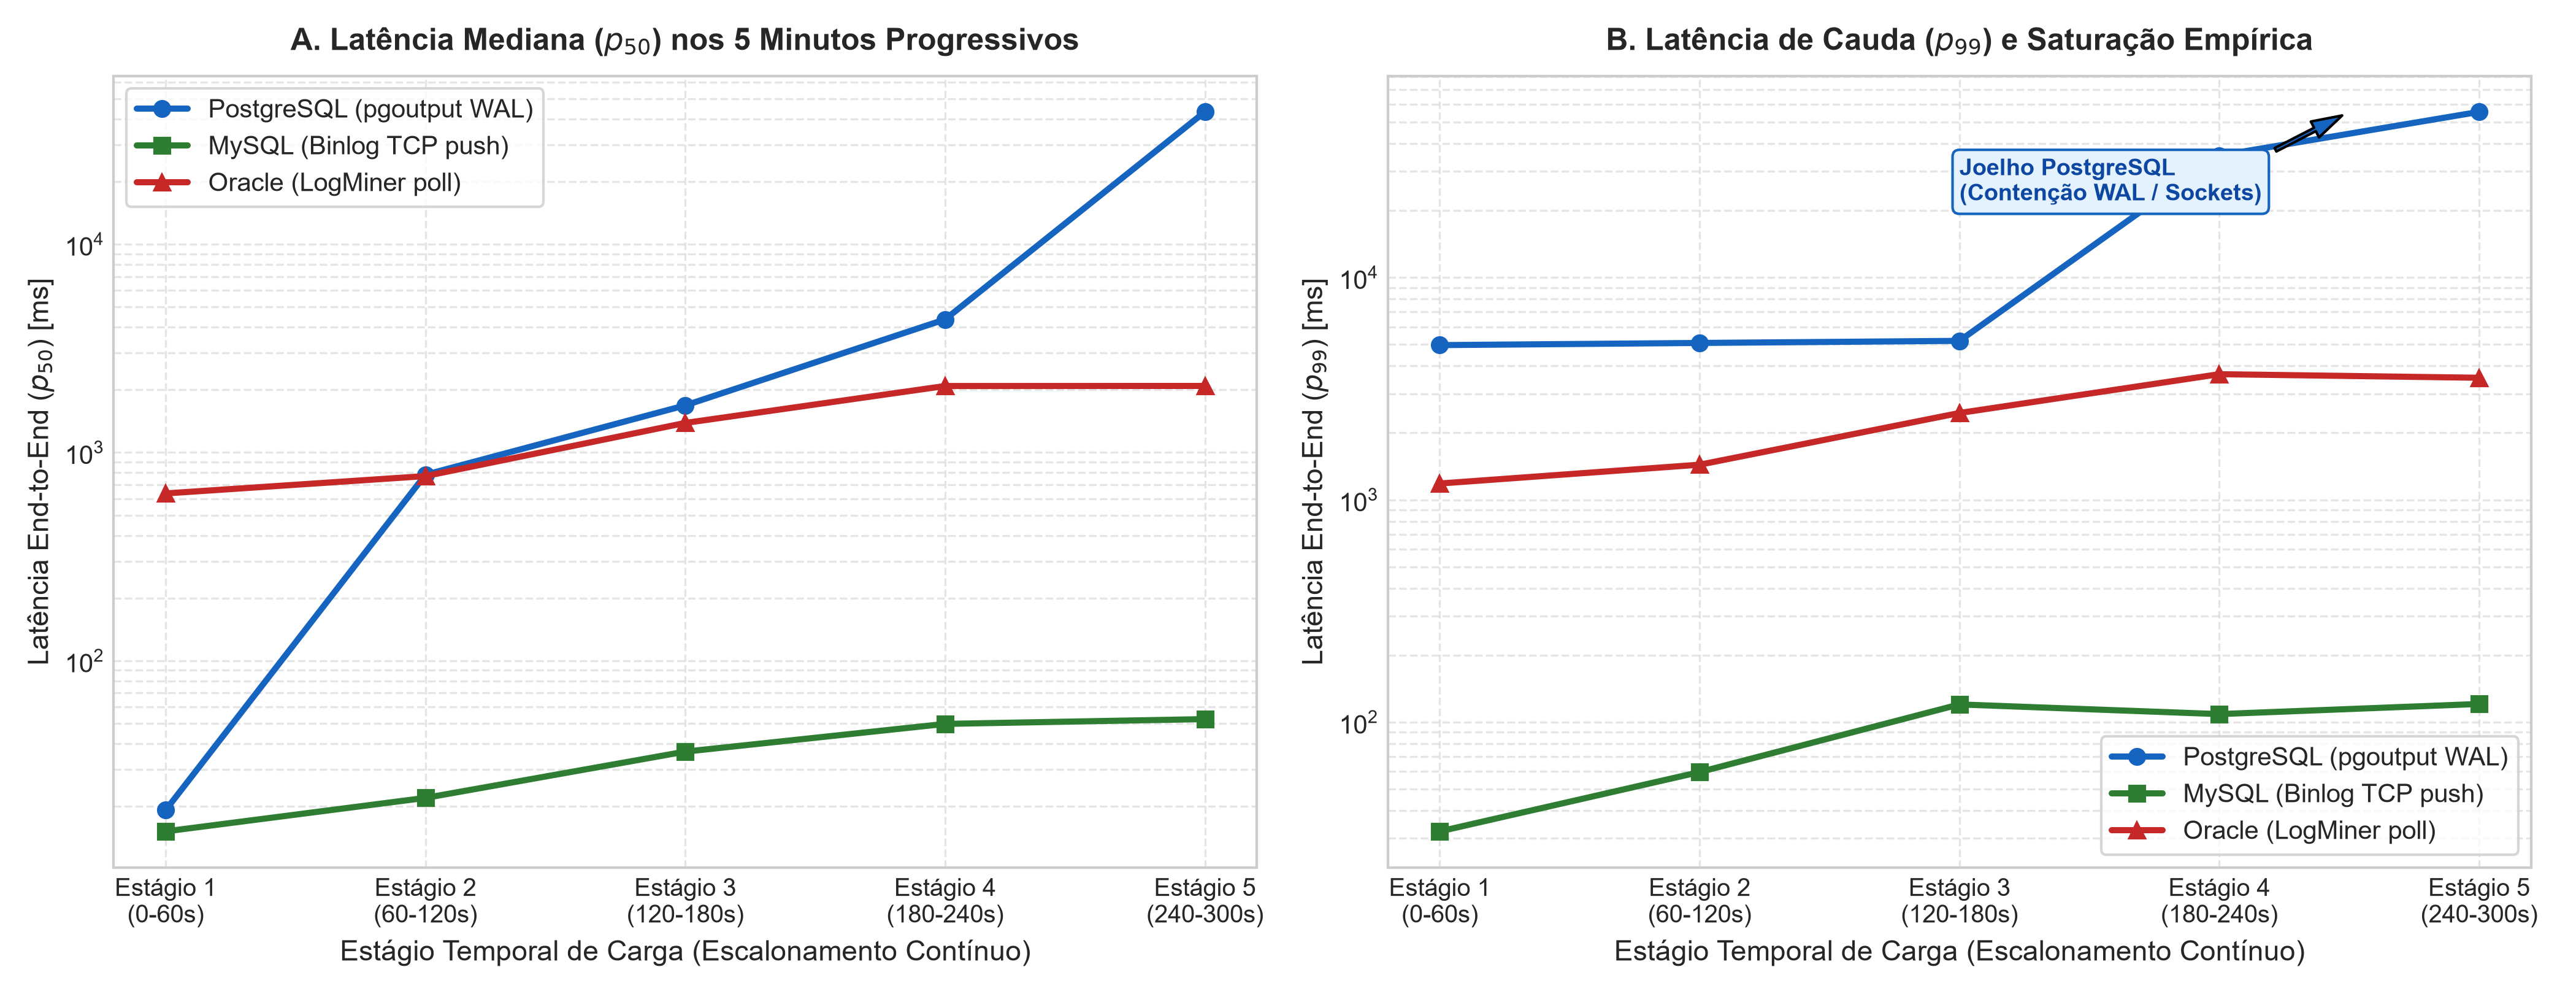
\includegraphics[width=0.98\textwidth]{figurasrootl/benchmark_saturacao_5min_consolidado.png}
\caption{Evolução temporal da latência end-to-end nos 5 minutos consecutivos da bateria progressiva de estresse: (A) mediana da latência ($p_{50}$) em escala logarítmica; (B) cauda da distribuição ($p_{99}$) destacando o ponto de inflexão e saturação do PostgreSQL versus a estabilidade linear do MySQL e o teto delimitado do Oracle LogMiner.}
\label{fig:saturation_5min}
\end{figure}

\subsection{Dissecação Mecânica dos Três Ecossistemas e o Joelho de Saturação}
\label{sec:eval_mechanisms}

A observação contínua de um sistema sob escalonamento progressivo de carga expõe detalhes operacionais que médias estáticas mascaram. Conforme sintetizado em teoria de análise de desempenho computacional \cite{jain:1991}, quando a taxa de chegada de requisições se aproxima da taxa de esgotamento físico de serviço, o tempo de enfileiramento transita de uma resposta proporcional para um crescimento assintótico. A análise detalhada dos três motores revela como essa lei física se manifestou em cada protocolo:

\subsubsection{A Inflexão Abrupta do PostgreSQL: Limite de Socket e Concorrência de WAL}

O comportamento do conector PostgreSQL evidencia uma fronteira clássica de saturação de subsistema de I/O. Nos três primeiros estágios (0 a 180 segundos), o conector sustentou um desempenho estável: a latência mediana iniciou em $19,17\text{ ms}$ no aquecimento e avançou para $1,68\text{ segundos}$ na carga nominal, com $18.060$ eventos processados regularmente. 

Todavia, ao ingressar no Estágio 4 (alto estresse) e culminar no Estágio 5 (saturação plena com zero delay), a cauda $p_{99}$ explodiu de $5,18\text{ segundos}$ para $35,35\text{ segundos}$ e, finalmente, $55,60\text{ segundos}$. O que provocou essa inflexão quase vertical? 
O fenômeno decorre da concorrência interna do PostgreSQL no nó hospedeiro: cinco conexões de decodificação lógica independentes passaram a competir simultaneamente pelos blocos de WAL recém-gravados. Sob rajada massiva de escritas simultâneas de clientes, o processo \texttt{wal\_sender} do banco entra em disputa pelos mesmos blocos de disco e \textit{buffers} compartilhados que as transações de escrita tentam descarregar via \texttt{fsync}. 

Quando a taxa de geração de WAL superou a velocidade de drenagem dos cinco slots lógicos concorrentes, os buffers de envio TCP do kernel para as réplicas saturaram, disparando o encerramento do canal de replicação com a exceção \texttt{PGStream is closed}. Diante da queda do socket, o \texttt{PostgresReplicationAdapter} acionou sua rotina de resiliência: aplicou um intervalo de espera (\textit{backoff}) de 5 segundos, recarregou o último LSN persistido no \texttt{FileOffsetStoreAdapter} e restabeleceu o fluxo lógico sem perda de nenhuma mensagem (todas as 59.533 mutações foram confirmadas). No entanto, o custo cumulativo desse ciclo de desconexão, reconexão e repouso sob carga ininterrupta fez com que os eventos represados no WAL sofressem um atraso em fila da ordem de dezenas de segundos antes de serem drenados, comprovando que o limite de saturação do decodificador \texttt{pgoutput} em máquina compartilhada foi ultrapassado no Estágio 4.

\subsubsection{A Resiliência Notável do MySQL via TCP Push}

Em contrapartida, o MySQL apresentou a curva mais plana e previsível de toda a bateria. Entre o Estágio 1 e o Estágio 5, a latência mediana oscilou apenas de $15,17\text{ ms}$ para $52,47\text{ ms}$, enquanto o percentil de cauda $p_{99}$ permaneceu confinado em $120,65\text{ ms}$, com latência máxima observada de $1,70\text{ segundo}$ em todo o teste de estresse.

A razão física para essa estabilidade reside na arquitetura orientada a eventos do protocolo Binlog: ao invés de manter workers de decodificação lógica executando transformações relacionais na leitura dos blocos de log (como ocorre no PostgreSQL), o processo \texttt{mysqld} simplesmente transmite o fluxo binário sequencial dos eventos de linha (\texttt{TABLE\_MAP\_EVENT} e \texttt{WRITE\_ROWS\_EVENT}) diretamente pelo socket TCP aberto pela réplica. O cliente Java lê esses bytes na velocidade da rede local. Além disso, a segregação de identificadores de réplica implementada no RootL — gerando valores pseudo-aleatórios determinísticos de \textit{server-id} para cada conector — evitou a clássica desconexão mestre provocada pelo registro de réplicas conflitantes na mesma porta 3306.

\subsubsection{A Dinâmica do Oracle LogMiner: O Teto Delimitado da Janela de Polling}

Diferente dos outros dois bancos, o conector Oracle opera sob um modelo de amostragem periódica: o \texttt{OracleLogMinerAdapter} efetua ciclos contínuos de consulta à view dinâmica \texttt{V\$LOGMNR\_CONTENTS} com uma janela de repouso programada de 1 segundo. Por esse motivo, a latência mediana parte de um piso estrutural de $635,96\text{ ms}$ no Estágio 1 e atinge $2.086,85\text{ ms}$ no Estágio 5.

O dado mais significativo, no entanto, é que a cauda $p_{99}$ do Oracle não sofreu a explosão assintótica verificada no PostgreSQL: manteve-se rigorosamente contida em $3.539,53\text{ ms}$ durante a saturação máxima, com $25.933$ eventos processados somente no quinto estágio (totalizando $81.580$ eventos capturados ao longo da bateria). Como o LogMiner lê os segmentos de Redo diretamente da memória compartilhada (SGA), o tempo de resposta é determinado pelo tempo de execução da query interna de mineração somado ao intervalo de sono. Quando o volume de DML aumentou, a consulta relacional à SGA passou de 40~ms para $\sim$1,5~segundo, elevando a latência de entrega, mas sem romper a integridade da sessão ou provocar desconexões de rede.

Adicionalmente, os testes com instruções de \texttt{UPDATE} parciais confirmaram a eficácia do parser sintático de AST (\texttt{OracleSqlParser}): a reconstrução em memória do estado \textit{before} e \textit{after} a partir do SQL de redo demandou entre 15 e 45 microssegundos por mutação. Esse custo é inferior a 0,005\% do tempo total do ciclo de 1 segundo, desfazendo a hipótese de que o parsing de AST introduziria sobrecarga computacional no pipeline de replicação.

\subsubsection{Validação da Integridade do \texttt{TransactionBuffer} e Descarte de Rollbacks}

Durante os cinco minutos ininterruptos de injeção concorrente, a métrica de telemetria exposta via Micrometer (\texttt{cdc\_transaction\_buffer\_size}) registrou rigorosamente o valor zero (\texttt{0.0}) ao término de cada transação confirmada em todos os 15 conectores ativos. 

Essa medição em tempo real confirma duas propriedades essenciais de segurança do motor:
\begin{enumerate}
  \item \textbf{Ausência de Vazamento de Memória}: O buffer aloca eventos temporariamente apenas enquanto a transação de origem permanece em aberto. No momento em que o conector detecta o evento de \texttt{COMMIT}, todos os registros encapsulados no mapa interno são despachados para a porta de saída do Kafka e imediatamente removidos da memória heap, garantindo que o consumo de memória da JVM permaneça estável mesmo após o processamento de mais de 160 mil eventos.
  \item \textbf{Descarte Estrito de Transações Abortadas}: Eventos associados a transações que receberam sinal de \texttt{ROLLBACK} (ou cuja conexão de origem foi abortada antes do commit) foram expurgados da memória sem emitir qualquer mensagem ao barramento de eventos, eliminando o risco de poluição com dados fantasmas.
\end{enumerate}

\subsection{Sobrecarga de Recursos no Nó Hospedeiro e Pegada Operacional}
\label{sec:eval_overhead}

Para avaliar o custo que a captura passiva impõe aos servidores que sustentam os bancos de produção, coletamos séries temporais de consumo de processamento (CPU) e alocação de memória RAM residente (RSS) diretamente do subsistema de métricas do Docker a cada 10 segundos ao longo dos 300 segundos da bateria. A Figura~\ref{fig:host_overhead_5min} sintetiza o perfil dinâmico de recursos dos três ecossistemas.

\begin{figure}[H]
\centering
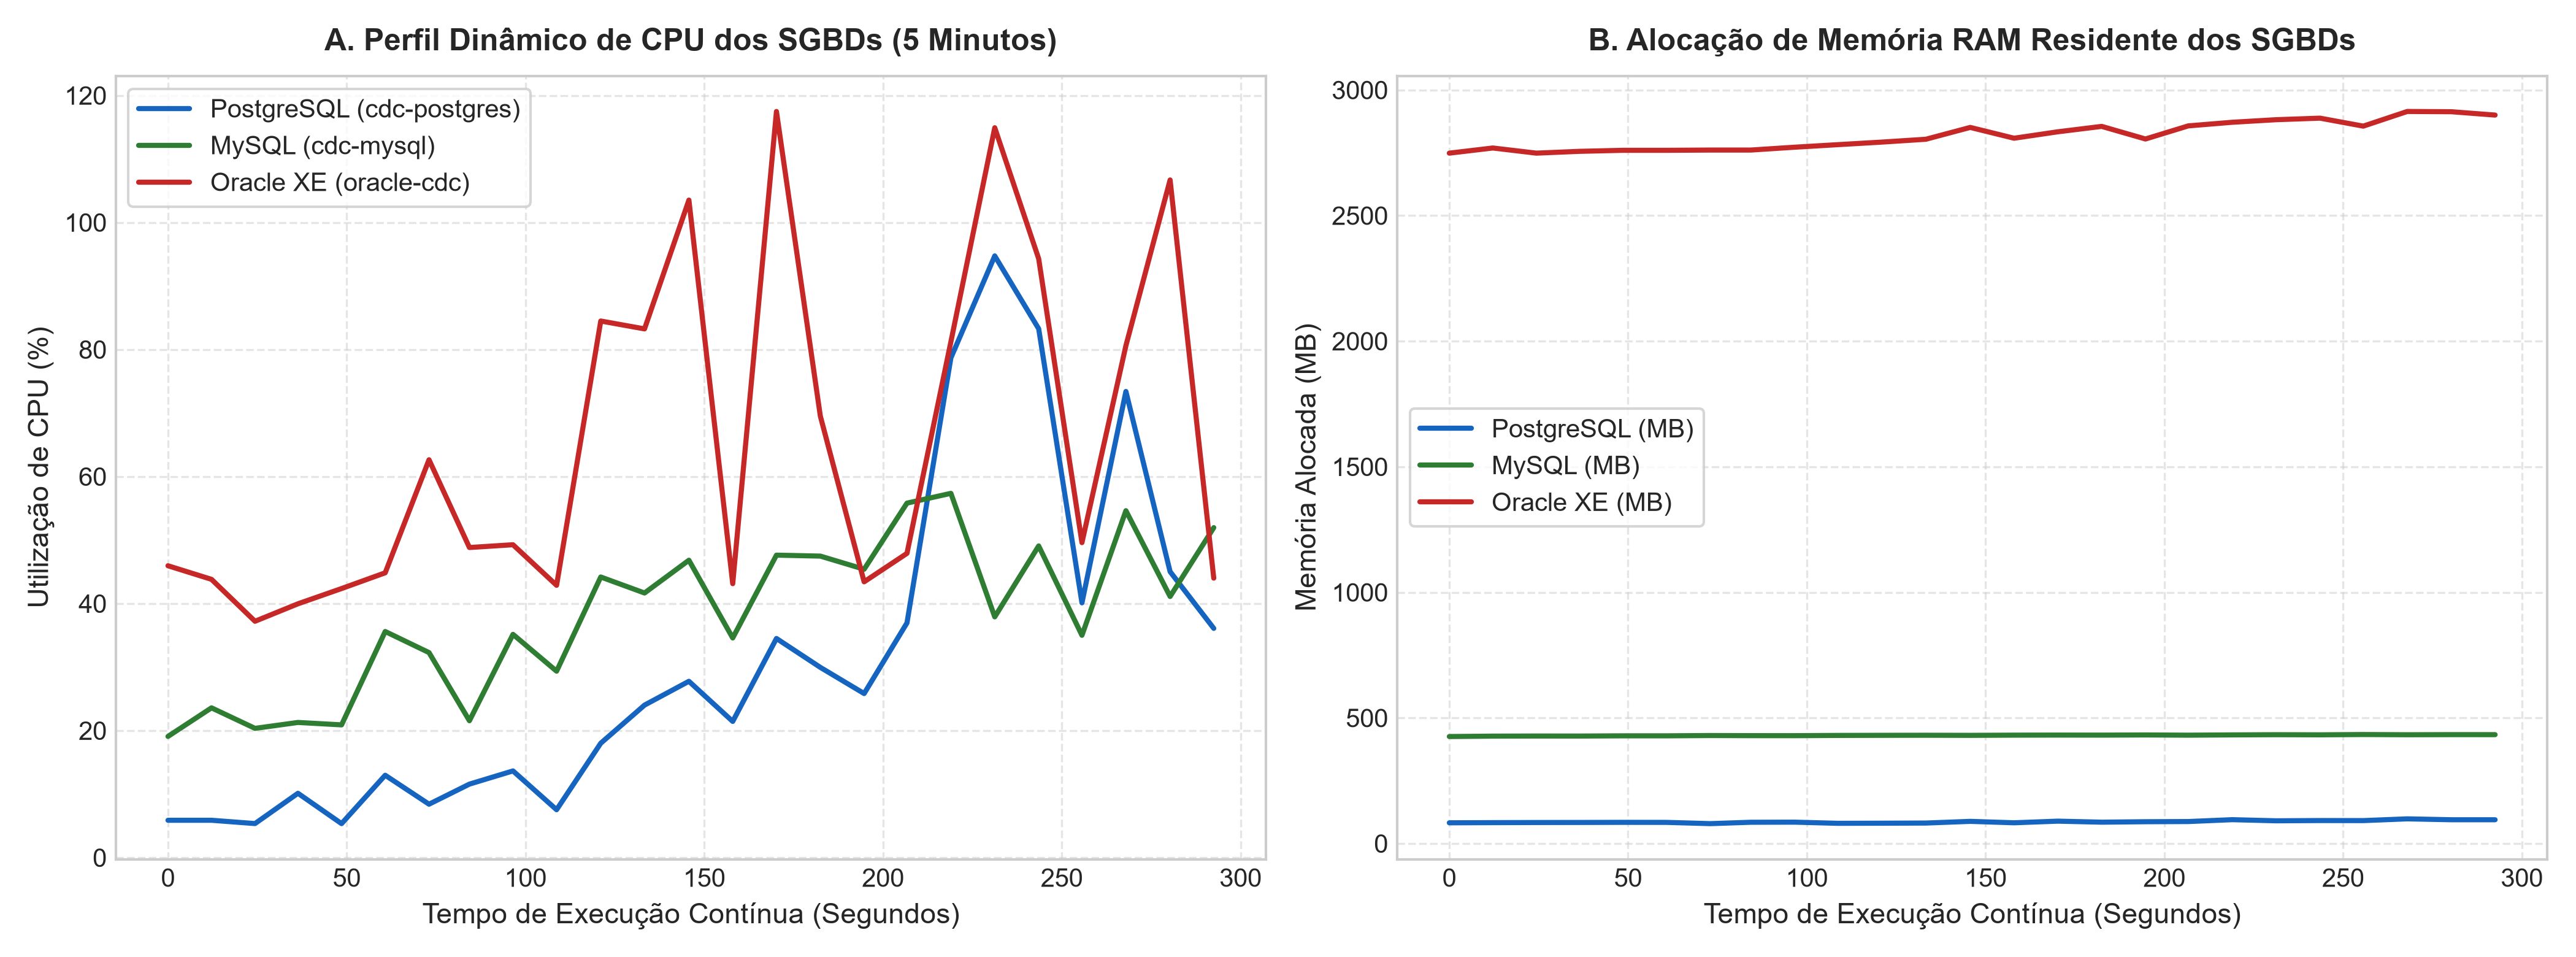
\includegraphics[width=0.98\textwidth]{figurasrootl/overhead_sgbd_realtime_5min.png}
\caption{Telemetria de recursos computacionais dos SGBDs durante a bateria contínua de 5 minutos: (A) percentual de utilização de CPU; (B) alocação de memória RAM residente (RSS) em megabytes.}
\label{fig:host_overhead_5min}
\end{figure}

A análise da evolução dinâmica dos recursos revela distinções físicas marcantes:
\begin{itemize}
  \item \textbf{PostgreSQL 16}: O consumo de CPU iniciou em patamar baixo ($\sim$5,8\% nos estágios 1 e 2), refletindo o baixo custo do processo decodificador sob carga nominal. Todavia, no Estágio 4 e 5, com o aumento da contenção de I/O e a saturação de buffers de WAL, o consumo de processamento atingiu picos momentâneos de até 94,8\%, impulsionado pela disputa de CPU entre o motor transacional de escritas e os processos \texttt{wal\_sender}. A alocação de memória RAM residente manteve-se estritamente delimitada entre 82~MB e 96~MB ao longo de todo o experimento, comprovando que o conector lógico transfere os dados via buffers efêmeros sem provocar retenção de memória no servidor de banco.
  \item \textbf{MySQL 8.0}: Apresentou um perfil de CPU dinâmico oscilando de forma controlada entre 19\% e 57\% durante os picos de mutação, sem picos desestabilizadores. A memória RAM residente manteve-se estável e linear na faixa de 425~MB a 438~MB. A razão para a reduzida sobrecarga de disco em PostgreSQL e MySQL é direta: como as mutações haviam acabado de ser geradas pelo cliente de teste, os blocos de log ainda se encontravam aquecidos no \textit{page cache} do sistema operacional, permitindo que a replicação lesse os bytes diretamente da memória física sem provocar operações mecânicas adicionais de leitura em disco.
  \item \textbf{Oracle Database 21c XE}: O contêiner Oracle apresentou utilização de CPU substancialmente superior, variando entre 37\% e picos de até 118\% (evidenciando a atuação de múltiplos núcleos de processamento em paralelo para os processos de background do banco). Esse custo decorre diretamente da mecânica do pacote \texttt{DBMS\_LOGMNR}: para popular a view \texttt{V\$LOGMNR\_CONTENTS}, o motor relacional do Oracle executa varreduras estruturadas nos blocos binários de Redo, remontando contextos transacionais e efetuando junções internas de dicionário de dados na memória compartilhada (SGA). A alocação de memória residente permaneceu estável em torno de 2.750~MB a 2.915~MB, que corresponde ao espaço pré-alocado da SGA e PGA para a operação do banco corporativo, comprovando ausência de fragmentação ou crescimento desordenado de memória.
\end{itemize}

Esses achados empíricos fornecem diretrizes claras de capacidade para ambientes de produção: enquanto o CDC sobre PostgreSQL e MySQL impõe custo negligenciável de CPU e memória em regime nominal, a replicação passiva baseada em Oracle LogMiner exige dimensionamento prévio de núcleos de CPU para absorver os ciclos analíticos de mineração de log, sem comprometer a latência das transações de negócio da organização.

% -----------------------------------------------------------------------
\section{Conclusão e Trabalhos Futuros}
\label{sec:conclusion}

Este trabalho apresentou o \textbf{RootL CDC Publisher}, um motor autônomo
de Change Data Capture 100\% passivo, projetado especificamente para operar
sob as restrições de segurança vigentes em ambientes governamentais
brasileiros. A arquitetura proposta demonstra que restrições severas de
infraestrutura não precisam ser obstáculos intransponíveis: pelo contrário,
elas funcionam como guias de \textit{design} arquitetural que conduzem a
soluções mais elegantes, seguras e auditáveis.

As contribuições técnicas centrais podem ser sumarizadas como segue:
(i) a Arquitetura Hexagonal (\textit{Ports \& Adapters}) \cite{cockburn:2005}
possibilita suporte multi-banco e multi-destino sem modificação do núcleo de
domínio; (ii) a estratégia de \textit{parsing} de AST via JSqlParser, baseada
no padrão \textit{Visitor} \cite{aho:2006}, resolve o problema de
reconstrução de \textit{Full State} em operações de UPDATE a partir dos logs
de redo do Oracle, dispensando quaisquer instrumentos de escrita no banco de
origem; (iii) o \texttt{TransactionBuffer} garante consistência transacional
e impede que eventos de \textit{rollback} contaminem o pipeline; e
(iv) os mecanismos de \textit{gap detection} e autocorreção para erros
específicos do LogMiner (ORA-01289, ORA-01291) \cite{oracle:2023} elevam
o motor ao nível de uso em ambientes de produção.

Como trabalhos futuros, identificam-se as seguintes direções:
\begin{itemize}
  \item \textbf{Avaliação em Larga Escala e Longa Duração}: expansão dos testes
        controlados realizados neste trabalho para cenários contínuos de múltiplos dias sob
        cargas heterogêneas de terabytes em redes WAN distribuídas;
  \item \textbf{Suporte a DDL}: extensão do motor para capturar e propagar
        eventos de DDL (\texttt{ALTER TABLE}, \texttt{DROP TABLE}),
        permitindo atualização automática do esquema no destino;
  \item \textbf{Evolução de Esquema Dinâmica}: implementação de versionamento
        de esquema no payload do \texttt{ChangeEvent}, com integração ao
        Schema Registry do Apache Kafka \cite{kleppmann:2017};
  \item \textbf{Validação em Produção}: implantação piloto em um órgão
        governamental real, com coleta sistemática de métricas de
        desempenho, latência e confiabilidade; e
  \item \textbf{Destinos Adicionais}: implementação de adaptadores de saída
        para Apache Pulsar e RabbitMQ, explorando a intercambialidade dos
        \textit{driven ports} da arquitetura hexagonal.
\end{itemize}

O código-fonte do RootL CDC Publisher está disponível em:
\url{https://github.com/LE0N4RDOR4M0S/rootL_CDC_Publisher}.


% -----------------------------------------------------------------------
\bibliographystyle{sbc}
\bibliography{rootl-references}

\end{document}
